\begin{figure*}[t]
  \centering
  \begin{subfigure}[b]{\appendixwidth\textwidth}
    \centering
    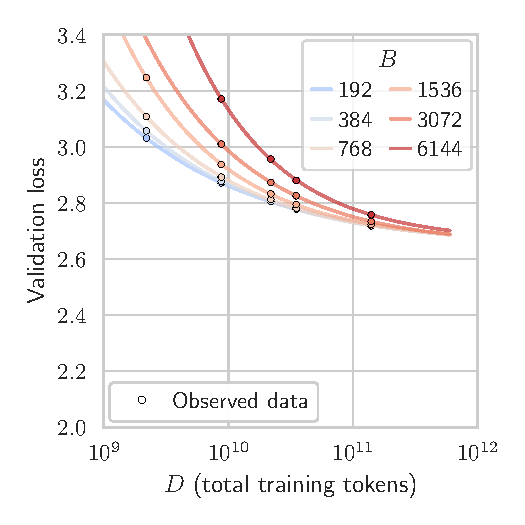
\includegraphics[trim={0.3cm 0.4cm 0.3cm 0.3cm}, clip, width=\linewidth]{pdffigs/241005.fitted_scale_law.gbs=multi.111M.pdf}
    \caption{111M scale}
    \label{fig:quad_cbs_111M}
  \end{subfigure}
  \hfill
  \begin{subfigure}[b]{\appendixwidth\textwidth}
    \centering
    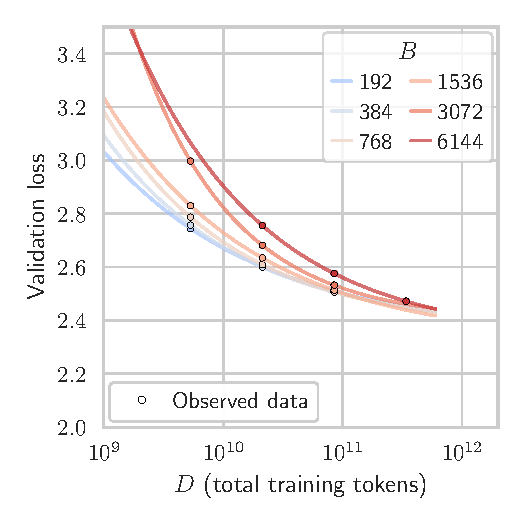
\includegraphics[trim={0.3cm 0.4cm 0.3cm 0.3cm}, clip, width=\linewidth]{pdffigs/241005.fitted_scale_law.gbs=multi.266M.pdf}
    \caption{266M scale}
    \label{fig:quad_cbs_266M}
  \end{subfigure}
  % Next row
  \begin{subfigure}[b]{\appendixwidth\textwidth}
    \centering
    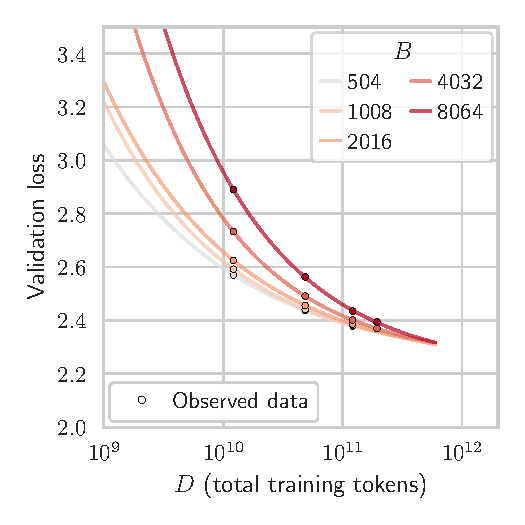
\includegraphics[trim={0.3cm 0.4cm 0.3cm 0.3cm}, clip, width=\linewidth]{pdffigs/241005.fitted_scale_law.gbs=multi.617M.pdf}
    \caption{610M scale}
    \label{fig:quad_cbs_617M}
  \end{subfigure}
  \hfill
  \begin{subfigure}[b]{\appendixwidth\textwidth}
    \centering
    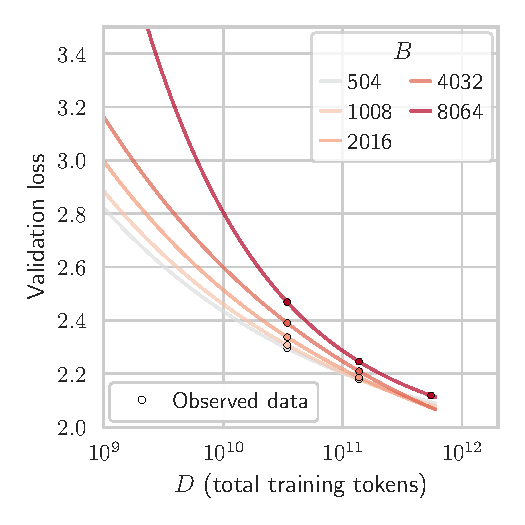
\includegraphics[trim={0.3cm 0.4cm 0.3cm 0.3cm}, clip, width=\linewidth]{pdffigs/241005.fitted_scale_law.gbs=multi.1.7B.pdf}
    \caption{1.7B scale}
    \label{fig:quad_cbs_1_7B}
  \end{subfigure}
  \caption{\textbf{Scaling laws in $D$ for computing $\cbs$}: Full set
    of $B$-specific power laws, for 111M to 1.7B scales, fitted after
    training models with different batch sizes, $B$, and dataset
    sizes, $D$, at each scale (empirical data from real training runs
    indicated by points).  From these power laws, we can compute the
    amount of data needed to reach any target loss, as illustrated in
    main paper \cref{fig:cbs_fitting}.\label{fig:quad_cbs_fitting}}
\end{figure*}
